\documentclass[border=30pt, multi, tikz]{standalone}
\usepackage{import}
\subimport{layers/}{init}
\usetikzlibrary{positioning, 3d}

% Define colors
\def\ConvColor{rgb:yellow,5;red,2.5;white,5}
\def\ConvReluColor{rgb:yellow,5;red,5;white,5}
\def\FcColor{rgb:blue,5;red,2.5;white,5}
\def\FcReluColor{rgb:blue,5;red,5;white,4}
\def\PoolColor{rgb:red,1;black,0.3}
\def\DropoutColor{rgb:magenta,1;black,2}
\def\ConcatColor{rgb:green,4;black,4}
\def\SoftmaxColor{rgb:magenta,5;black,7}
\def\SumColor{rgb:blue,5;green,15}

\begin{document}
\begin{tikzpicture}
\tikzstyle{connection}=[ultra thick,every node/.style={sloped,allow upside down},draw=black,opacity=0.7]
% ----- INPUT IMAGE -----
\node[canvas is zy plane at x=0] (xray) at (-1.6,0,0) {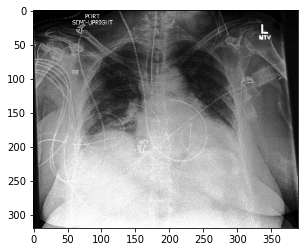
\includegraphics[width=7.5cm,height=7.5cm]{lung.png}};
% ----- IMAGE PATH -----
\pic[shift={(0,0,0)}] at (0,0,0) {Box={name=conv1, caption=Conv1\\(7x7), xlabel={{"64", ""}}, fill=\ConvColor, height=30, width=1, depth=30}};
\pic[shift={(1.6,0,0)}] at (conv1-east) {Box={name=pool1, caption=MaxPool\\(3x3), fill=\PoolColor, height=28, width=1, depth=28}};

\pic[shift={(1.6,0,0)}] at (pool1-east) {RightBandedBox={name=res1, caption=ResBlock1\\(256), xlabel={{"","","256"}}, fill=\ConvColor, bandfill=\ConvReluColor, height=24, width={1.5,1.5, 1.5}, depth=24}};
\pic[shift={(1.6,0,0)}] at (res1-east) {RightBandedBox={name=res2, caption=ResBlock2\\(512), xlabel={{"","","","512"}}, fill=\ConvColor, bandfill=\ConvReluColor, height=22, width={1.5,1.5,1.5,1.5}, depth=22}};
\pic[shift={(1.6,0,0)}] at (res2-east) {RightBandedBox={name=res3, caption=ResBlock3\\(1024), xlabel={{"","","","","","1024"}}, fill=\ConvColor, bandfill=\ConvReluColor, height=20, width={1.5,1.5,1.5,1.5,1.5,1.5}, depth=20}};
\pic[shift={(1.6,0,0)}] at (res3-east) {RightBandedBox={name=res4, caption=ResBlock4\\(2048), xlabel={{"","","2048"}},fill=\ConvColor, bandfill=\ConvReluColor, height=18, width={1.5,1.5,1.5}, depth=18}};
\pic[shift={(1.6,0,0)}] at (res4-east) {Box={name=imgemb, caption=\shortstack{\textbf{2048-d}\\embedding}, fill=\FcColor, height=10, width=1, depth=8}};

% ----- CLINICAL FEATURE PATH -----
\pic[shift={(0,-6,0)}] at (0,0,0) {Box={name=tabinput, caption=\shortstack{Structured\\Data}, fill=\FcColor, height=10, width=1, depth=10}};
\pic[shift={(1.8,0,0)}] at (tabinput-east) {Box={name=knn, caption=kNN\\Imputer, fill=\DropoutColor, height=6, width=1, depth=6}};
\pic[shift={(2.2,0,0)}] at (knn-east) {RightBandedBox={name=mlp, caption=MLP\\(128\textrightarrow64), xlabel={{"128","64"}}, fill=\FcColor, bandfill=\FcReluColor, height=8, width={2.5,2.5}, depth=8}};
\pic[shift={(2.2,0,0)}] at (mlp-east) {Box={name=tabemb, caption=\shortstack{\textbf{64-d}\\embedding}, fill=\FcColor, height=6, width=1, depth=6}};

% ----- FUSION AND CLASSIFIER -----
\pic[shift={(2.5,-3,0)}] at (imgemb-east) {Ball={name=concat, fill=\SumColor, opacity=0.6, radius=1.5, logo=$\oplus$}};
\pic[shift={(2,0,0)}] at (concat-east) {RightBandedBox={name=fc1, caption=\shortstack{Classifier\\(64 hidden)}, xlabel={{"64"}}, fill=\FcColor, bandfill=\FcReluColor, height=8, width={1.5,1.5}, depth=8}};
\pic[shift={(2,0,0)}] at (fc1-east) {Box={name=output, caption=\shortstack{Softmax\\(3 classes)}, fill=\SoftmaxColor, height=6, width=1, depth=6}};

% ----- CONNECTIONS -----
\draw [connection] (conv1-east) -- (pool1-west);
\draw [connection] (pool1-east) -- (res1-west);
\draw [connection] (res1-east) -- (res2-west);
\draw [connection] (res2-east) -- (res3-west);
\draw [connection] (res3-east) -- (res4-west);
\draw [connection] (res4-east) -- (imgemb-west);
\draw [connection] (imgemb-east) -- (concat-west);

\draw [connection] (tabinput-east) -- (knn-west);
\draw [connection] (knn-east) -- (mlp-west);
\draw [connection] (mlp-east) -- (tabemb-west);
\draw [connection] (tabemb-east) -- (concat-south);

\draw [connection] (concat-east) -- (fc1-west);
\draw [connection] (fc1-east) -- (output-west);

\end{tikzpicture}
\end{document}
